\documentclass[10pt,b5paper,tombo,openany]{jsbook}

\usepackage[dvipdfmx]{graphicx}
\usepackage[dvipdfmx]{color}
\usepackage{listings}
\usepackage{inconsolata}
\usepackage{url}
\usepackage{titlesec}
%\usepackage{setspace}
%\usepackage{wrapfig}

\lstset{basicstyle={\small\ttfamily}}
\lstset{frame=single}
\lstset{breaklines=true}
\lstset{lineskip=-1.5pt}
\lstset{framesep=6pt}

\renewcommand{\kanjifamilydefault}{\gtdefault}
\renewcommand{\familydefault}{\sfdefault}
%\renewcommand{\contentsname}{}
%\renewcommand{\baselinestretch}{1.1}

\definecolor{gray75}{gray}{0.75}
\titleformat{\chapter}[hang]{\Huge\bfseries}{\thechapter\textcolor{gray75}{|}}{0pt}{\Huge\bfseries}

\begin{document}
\chapter{Big-Tent解説}

\section{CloudKitty}
\begin{description}
	\item[wiki:] \url{https://wiki.openstack.org/wiki/CloudKitty}
	\item[Document:] \url{http://docs.openstack.org/developer/cloudkitty/}
\end{description}
Rating-as-a-serviceと説明されていますが、課金管理をしてくれます。

Ceilometerは確かにメトリクスを計測してくれるのですが、課金に関してはそのスコープ外でした。課金のもととなるデータ(collector)、課金ポリシー(rating pipeline)、課金情報の保管(storage)、書き出し(writers)から構成されています。複数のコレクターや書き出しフォーマットを選ぶことができます。

\section{Congress}
\begin{description}
	\item[wiki:] \url{https://wiki.openstack.org/wiki/Congress}
\end{description}

\section{Designate}
\begin{description}
	\item[wiki:] \url{https://wiki.openstack.org/wiki/Designate}
\end{description}


\includegraphics[width=0.5\textwidth]{img/logo-designate.pdf}

みんな大好きDNSのサービスです。
\begin{itemize}
	\item ドメインとレコードの管理ができるAPIの提供
	\item マルチテナントのサポート
	\item NovaやNeutronと連携してレコードの自動追加
\end{itemize}
いまのところPowerDNSとBIND9をインストール時点でサポート。プラグイン型式で追加も可能のようです。

\section{Dragonflow}
\begin{description}
	\item[wiki:] \url{https://wiki.openstack.org/wiki/Dragonflow}
	\item[Document:] \url{http://docs.openstack.org/developer/dragonflow/distributed_dragonflow.html}
\end{description}
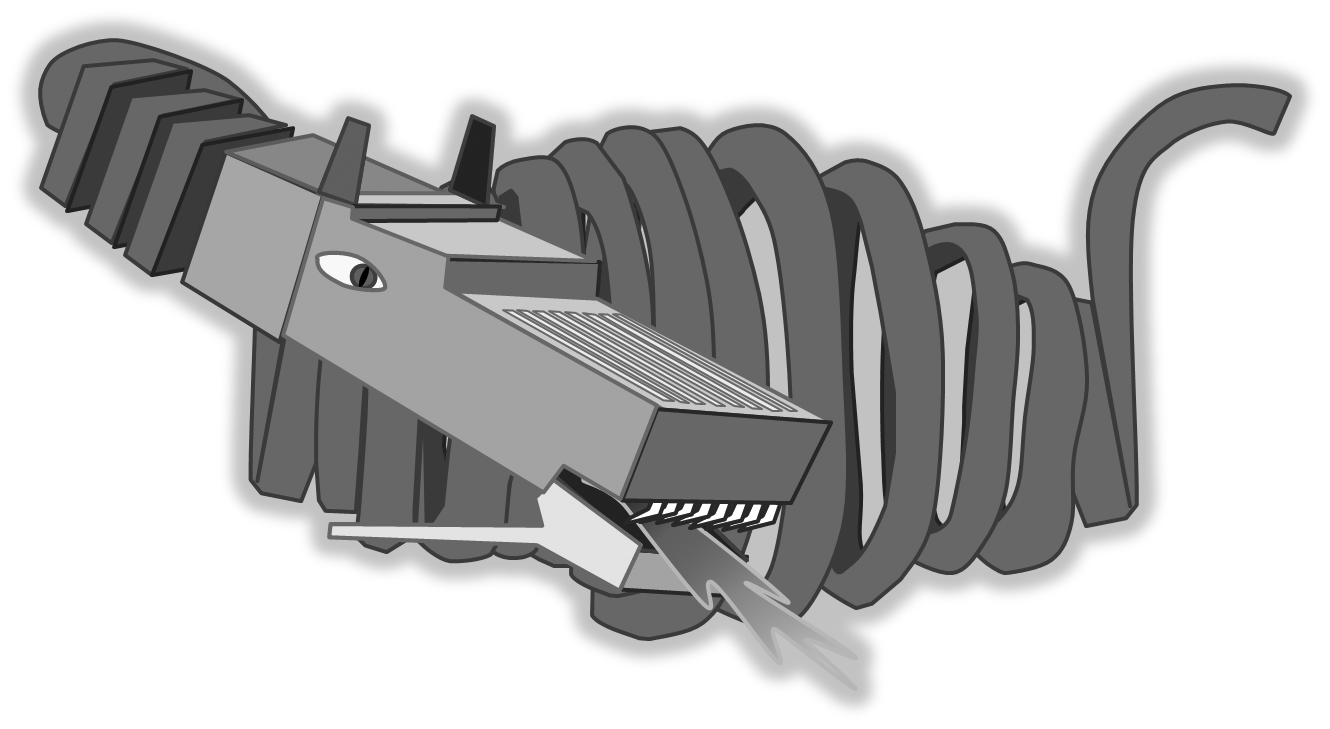
\includegraphics[width=0.5\textwidth]{img/Df_logo.png}

\section{Freezer}
\begin{description}
	\item[wiki:] \url{https://wiki.openstack.org/wiki/Freezer}
\end{description}


\includegraphics[width=0.5\textwidth]{img/freezer_logo.png}

バックアップサービスです。複数のOSをサポートし(Linux・Windows・OSX・*BSD)、ブロックストレージのバックアップやファイルシステムの差分バックアップを可能にすることが目標です。また、指定時間でのバックアップやジョブの同期など、バックアップスケジューリングもスコープに含みます。

\section{Karbor}
\begin{description}
	\item[wiki:] \url{https://wiki.openstack.org/wiki/Karbor}
\end{description}
旧Smaugです。WikiにはOpenStackデプロイのデータとメタデータを保護するもの、あるいはKeystoneのプロジェクト下にあるものの保護、と書いてありますがこれだけではどうにもピンときません。

例えば以下のようなアプリケーションがあったとします。

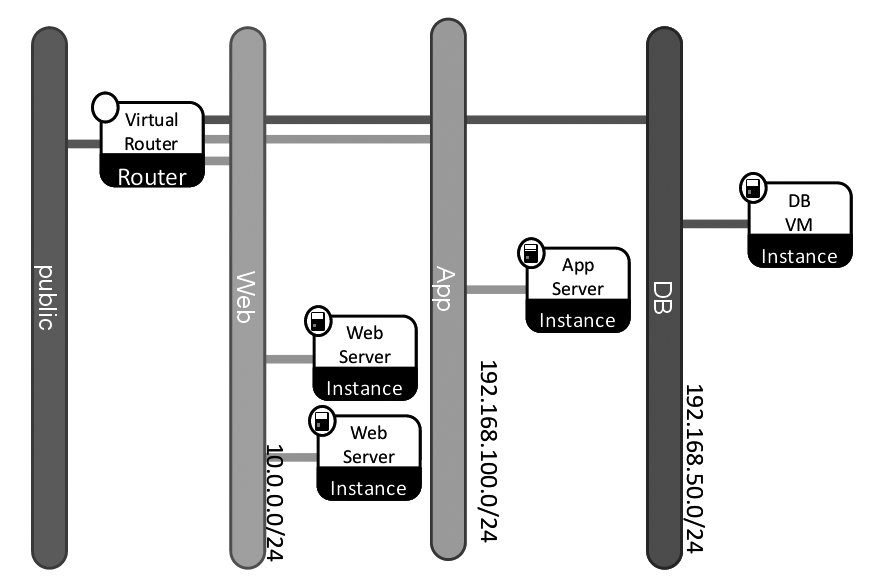
\includegraphics[width=\textwidth]{img/Smaug-sample-application.png}

このアプリケーションをシステムまるごと保存し、変更されたことを検知したいとします。このシステムを説明すると
\begin{itemize}
	\item DBインスタンスは1つで、DBネットワークに接続されている
	\item DBネットワークはRouter配下にある
	\item Appインスタンスは1つで、Appネットワークに接続されている
	\item AppネットワークはRouter配下にある
	\item Webインスタンスは2つあり
\end{itemize}
などなど、これらの情報を保存しておくことになります。

Karborではこれを依存グラフとして表現します

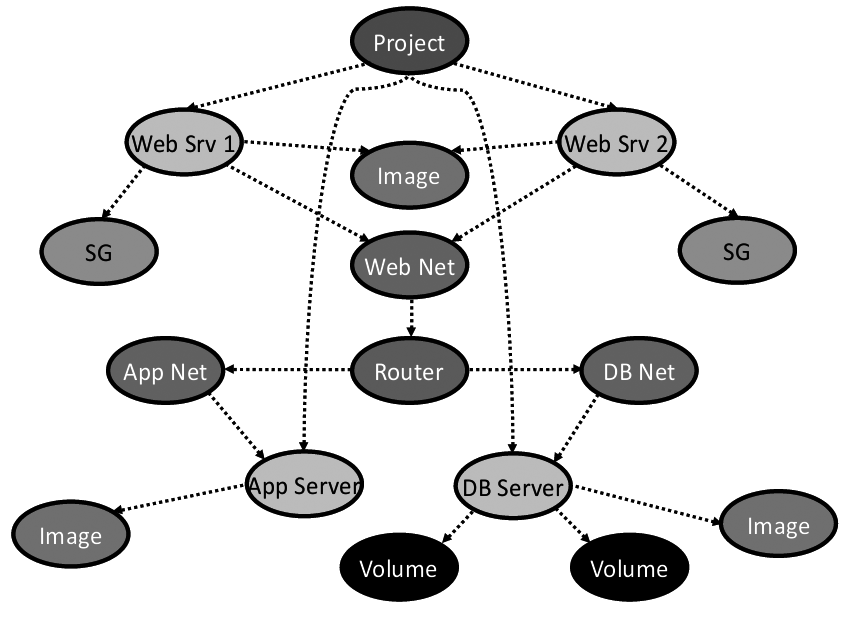
\includegraphics[width=\textwidth]{img/Smaug-dependency-graph.png}

\section{Kolla}
\begin{description}
	\item[wiki:] \url{https://wiki.openstack.org/wiki/Kolla}
\end{description}
OpenStackのコンポーネントをDocker化しようというプロジェクトです。OpenStackのAPIサーバーはImmutableなものとして扱うことが容易なので、すでにコンテナを使っている人も多いのではないかと思います。MissionにはOpenStackデプロイの簡素化や素早い増強ができるようにするとあります。

特にカスタマイズしなくても動くようなイメージを目指しているようですが、DockerfileをJinja2のテンプレートになっているのでカスタマイズが可能です。ソースコードからのインストール、RDOやUbuntuのリポジトリを使ったインストールの両方をサポートしています。

\section{Kuryr}
\begin{description}
	\item[wiki:] \url{https://wiki.openstack.org/wiki/Kuryr}
\end{description}
コンテナ用に設計されたネットワークプロジェクトです。もとはNeutronのサブプロジェクトでしたが、分離されました。コンテナに関しては長らくすったもんだを繰り返していましたが、ネットワークはKuryrになんとか落ち着いていきそうです。コンテナ自体はMagnumで落ち着きそうですし、OpenStackとコンテナはなんとか落としどころを見つけたのでしょうか。そもそも、仮想マシン(インスタンス)とコンテナではライフサイクルが違う、ということに無理があったそうで。

ところで、どう発音すればよいのかは謎である。

\chapter{あとがき}
\end{document}
